\chapter{依存句法分析 \\ Dependency Parsing}

\small{讲师:Christopher Manning, Richard Socher}

\small{作者:Lisa Wang, Juhi Naik, and Shayne Longpre}

\small{讲义来源:\cite{04-this_notes} 额外参考:\cite{04-this_slides}}

% 句法分析(Parsing, Syntax Analysis)就是1.句子由词语组成,2.词语具有语法功能。

% \begin{multicols}{2}

\section{依存语法和依存结构 \\ Dependency Grammar and Dependency Structure}

\subsection*{成分语法和依存语法 \\ Constituency Grammar and Dependency Grammar}

用树状结构表示句子语法结构的想法是自然的,形成的树称为句法树(Parse Tree)。编译原理中的句法树展示形式语言的语法结构,而NLP中的句法树展示自然语言的语法结构。
常用的句法树结构有两种:成分语法(Constituency Grammar)和依存语法(Dependency Grammar)。

成分语法使用嵌套表示句子语法结构,和编译原理中基于产生式的文法很像。各级语法层次通过规约向上整合,形成句子的不同成分(Nested Constituent),并构成句子。本节不涉及这个概念,欲详细了解可以参考\ref{Constituency Grammar},并建议参考\cite{04-phrase-struct-gram}和\cite{04-this_slides}。

依存语法展示了词之间的二元不对称关系,即依存关系,用三元组表示为$(Head, r, Dependent)$,两个实体分别指代被依赖者和依赖者;用单向弧表示为$Head\stackrel{r}{\to}Dependent$.以下简单列举几种依存关系:

\begin{itemize}
    \item 修饰关系,某个词修饰另一个词。依赖者是修饰词(Modifier),被依赖者是被修饰词(Governor)。比如the beautiful girl,修饰词是beautiful,被修饰词(主语)是girl,所以beautiful依存于girl.
    \item 主次关系,一系列词具有相同地位,用第一个词占根节点位;或者某个成分有同位语,此时同位语依存于这个词。依赖者是下级(Inferior),被依赖者是上级(Superior)。
    \item 从属关系,某个词从属另一个词。依赖者是从属词(Subordinate),被依赖者是支配词(Regent)。
\end{itemize}

在具体分析句子的时候,一般先通过语法关系定义依存的不同种类,再确定每一处依存属于什么种类。
\cite{04-blog1}给出了更多、更精确的依存关系实例。从中可见,依存关系基本上是根据语法关系(主谓宾,同位语等)和句子成分(主语、介词宾语、同位语等)定义或设计的。然而,依存关系并不像成分语法那样一丝不苟地遵循自然语言语法设计关系:依存关系不强求和自然语言语法的严格对应,而是优先从方便计算机处理、方便标注数据等等因素来考虑,比如保证定义明确无歧义等等。因此,依存语法在确切语言学对应、关系直观性等human-friendly的方面可能稍逊于成分语法,但在表示难度、处理难度等属于process-friendly方面的因素表现更优。因此,目前大部分的句法分析数据集都是基于依存分析搭建的,而大多数较为成功的模型也是基于依存分析数据集提出的。

在依存的确切种类定义好之后,依存分析问题就是一个clearly-defined的计算机问题了。现在已经有了一些解决依存分析的工具,\cite{04-blog2}中介绍了一些应用实例。

\subsection{依存句法分析 \\ Dependency Parsing}

\subsubsection{依存树 \\ Dependency Tree}

依存树(Dependency Tree)就是以一个树状结构表示句子内部所有词的依存关系。在依存树中,依赖者作为被依赖者的子节点,通过依存关系连成树(有向图),如图\ref{04-tree}所示。

\begin{figure}[!htbp]
\centering
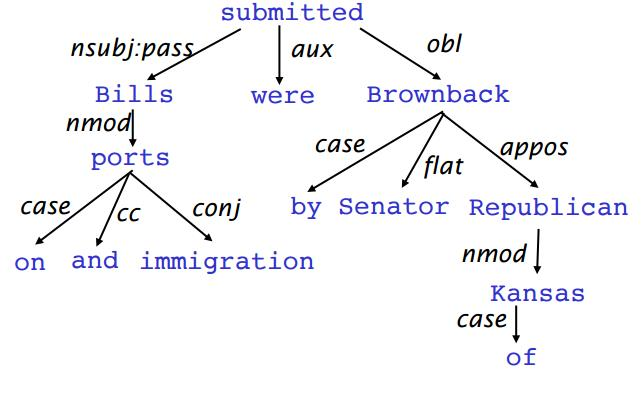
\includegraphics[width = 0.6\textwidth]{chap-04/04-01.jpg}
\caption{句子“Bills on ports and immigration were submitted by Senator Brownback, Republican of Kansas”的依存分析树。被依存者指向依存者,有向边上标识的属性是依存关系类型。}
\label{04-tree}
\end{figure}

有的时候会设置一个空节点充当这棵树的根节点,从而使句中的每一个词都依存于某个词。此时,可以用$S = (w_0w_1\cdots w_n)$表示一个句子,其中$w_0$是位于句首的空词语。
另外,在这种情况下,可以用两个和原句等长的序列表示依存树,一个序列确定被依赖词,一个序列确定是哪个关系。依存关系树可以用这种方式便利地表达出来。

\textbf{依存分析和句法分析的区别}

句法分析的核心是一步一步地解释句子展开成哪些成分,这些成分属于什么类型,然后再继续展开这些成分,自顶向下地把句子结构讨论清楚,并通过诸层次的展开关系来描述句子语法结果;而依存的分析方式并不是自顶向下的,也不需要把词汇本身的概念抽象出来,只是单纯展示句子中词语和词语之间的关系。
如前文所述,依存分析的结构更适合计算机处理\footnote{如上文所述,树状结构可以用两个序列表示,比嵌套结构表示起来方便一些,从而易于融入到通用的模型中。},同时也为人类保留了数据集的可读性(依存树也有一定的人类可读性),所以目前相对通常的句法分析/短语结构文法分析有优势。
关于短语结构文法/句法分析和依存语法分析的区别,建议阅读\cite{04-cnblogs2},讲的很详细。\cite{04-blog1}也点明了两者的区别。

关于自然语言的语法结构分析,还有很多新颖或实用的方法,比如普遍文法(或通用文法,Universal Grammar),旨在分析不同语言之间的共性成分,从而创建一个可以处理多种语言的大一统系统\footnote{相关资料可参考 \cite{04-uni1, 04-uni2, 04-uni3, 04-uni4}。}。

\subsubsection{依存句法分析的任务 \\ The Dependency Parsing Problem}

依存句法分析的任务是,输入句子$S$,输出依存句法树$G$. 这个任务分两部分(by Kuebler):

\begin{enumerate}
    \item 学习:给定数据集$D$(句子+句法树),训练模型$M$;
    \item 句法分析:使用这个模型进行预测,$G = M(S)$.
\end{enumerate}

在这方面,目前最流行的方法肯定是深度方法。

\subsection{基于状态转移的依存分析 \\ Transition-Based Dependency Parsing}

Transition-Based是一种做依存分析的思想,具有如下特点:

\begin{itemize}
    \item 数据集:每个句子的标签是从这个句子一步一步解析成依存分析树的状态转换序列。
    \item 模型效果:对于训练好的模型,输入句子当前的解析状态,输出下一个解析状态。所以预测模型是 一步一步地把整个句子的依存分析树解析出来。
\end{itemize}

因为依存分析的数据集在大多数情况下并不基于一个文法,所以不能给出一个明确的规约-展开规则,所以大部分Transition-Based的模型也并不需要依赖一个特定文法\footnote{也有基于成分分析搭建的模型,通过学习学到文法规则的使用策略(在给定的一组产生式中,在什么情况下优先用哪个产生式推导),然后通过这个策略逐步预测句子的推导过程。这种模型大多很麻烦,在此不多介绍。}。

\subsection{基于贪心方法的状态转移依存分析 \\ Greedy Deterministic Transition-Based Parsing}

根据上一节提出的Transition-Based思想,介绍(Nivre, 2003)模型,Nivre在2009年发表的综述\cite{04-NivreP}给出了这个模型的明确形式化定义。
对于用Transition-Based模型解决依存分析,这个模型实际上是将问题完全形式化,明确定义了Transition-Based模型应该具有的形式。

(Nivre, 2003)并不基于文法,而是基于一个有存储的状态机\footnote{形式语言的定义有两种主要途径,用文法定义或用状态机定义。\cite{04-tj}},定义如下:

\textbf{状态}

符合$c = (\sigma, \beta, A)$的三元组。其中:

\begin{itemize}
    \item $\sigma$表示一个栈,内部存储的元素是句子里的单词。
    \item $\beta$表示一个缓冲区,存储句子里的单词,对应尚未读入的单词。
    \item $A$表示句子中已经解析出来的依存关系的集合,其内部的元素形式为$(w_i, r, w_j)$,表示目前已经知道句子中$w_i, w_j$这两个词语之间具有$r$关系。
\end{itemize}

\textbf{初始状态和终止状态}

\begin{itemize}
    \item 初始状态:状态机只读入了句首的空单词,其他单词都还没读入,也没有任何依存关系被解析出来。
    $c_0 = ([w_0]_\sigma, [w_1, \cdots, w_n]_\beta, \emptyset)$.
    \item 终止状态:所有单词都读入,且栈中只剩根节点(特地加入的空节点,位于句首)的状态。
    $F = \{c_f\}, c_f = ([w_0]_\sigma, []_\beta, A)$.
\end{itemize}

\textbf{转移}

(Nivre, 2003)定义了三种状态转移:

\begin{itemize}
    \item $Shift$:在缓冲区非空的情况下,将缓冲区的第一个单词入栈。
    $(\sigma, w_i|\beta, A)\to(\sigma|w_i, \beta, A)$.
    \item $Left-Arc_r$:解析出依存关系$(w_j, r, w_i)$,其中$w_j$是栈顶,$w_i$是栈顶的第二个元素。在添加这个依存之后,$w_i$出栈。要求栈内至少有两个元素,且$w_i$不能为根节点。
    $(\sigma|w_i|w_j, \beta, A)\to(\sigma|w_j, \beta, A|\{r(w_j, w_i)\})$.
    \item $Right-Arc_r$:解析出依存关系$(w_i, r, w_j)$,其中$w_j$是栈顶,$w_i$是栈顶的第二个元素。在添加这个依存之后,$w_j$出栈。要求栈内至少有两个元素,且$w_i$不能为根节点。
    $(\sigma|w_i|w_j, \beta, A)\to(\sigma|w_i, \beta, A|\{r(w_i, w_j)\})$.
\end{itemize}

不难发现,对于任意一种状态,对其进行上述三种变换中的一种,所能得到的状态是唯一的:三种变换都是单值函数。也就是说,在给定当前状态时,Transition-Based模型用于在三种变换中正确决策。本节标题中提到的“贪心”正是点明这一点,模型不断对下一步转移进行判断,然后转移到下一个状态,至终止状态为止。

Nivre的工作还有很多,他自己在2019年也进行了总结,可以参考\cite{04-NivrePaper, 04-NivreSlides}.

\subsection{神经依存分析 \\ Neural Dependency Parsing}

本节在上一节基于贪心策略的Transition-Based模型基础上,介绍神经网络/机器学习/深度学习在其中的应用。如上一节所述,基于贪心策略的模型只需要在给定当前状态时做出下一步转移的决策(这实质上是一个分类问题),依决策移动到下一个状态,并最终解析出整个句子的依存关系。
在深度学习时代,我们在预测下一步转移时使用神经网络做分类,模型分为如下两步:

\textbf{特征选择}

基于特征选择的依存分析模型称为Feature-Based Discriminative Dependency Parsers,这类模型不直接用状态的完整信息做分类,而是通过一些预先定义的规则提取部分特征,并只参考这些特征的信息进行分类。在分类环节也不一定只使用神经网络模型,可能会基于一些简单统计或其他模型。

特征选择的环节就是在给定当前状态下,模型按规则从状态中提取若干特征,再根据特征形成模型的输入向量。一般提取的特征包括:

\begin{itemize}
    \item $S_{word}$:句子中的部分单词,用词向量的形式表示。这些单词一般是栈顶的几个单词或缓冲区即将被读入的前几个单词。使用单词的个数记为$n_w$.
    \item $S_{tag}$:一部分单词对应的词性(Part of Speech, POS)标签。使用词性标签的个数记为$n_t$.
    \item $S_{label}$:句子中存在的部分依存关系。前文提到,可以用两个和原句等长的序列表示句法树,一个序列确定被依赖词,一个序列确定是哪个关系;所以在此处,对于特定词语的依存关系,也用“被依存词+依存关系类型”来表示。关系的个数记为$n_l$.
\end{itemize}

\begin{figure}[!htbp]
\centering
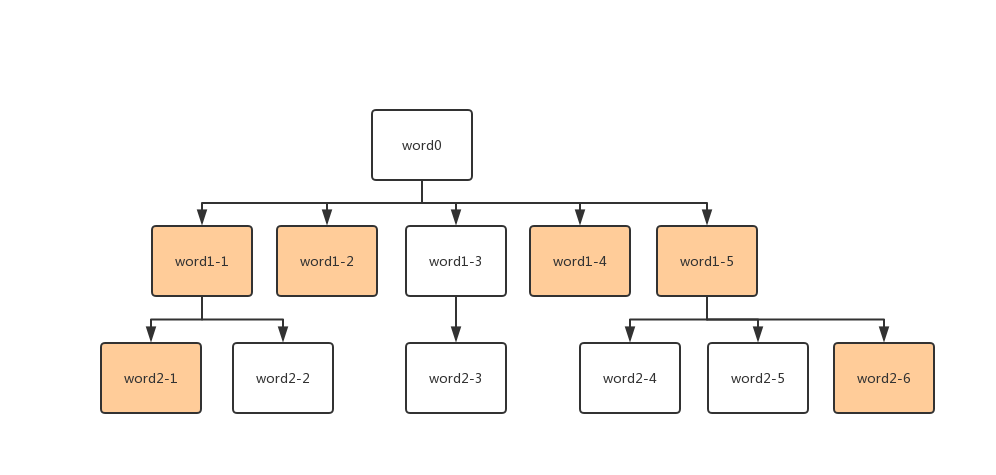
\includegraphics[width = 0.7\textwidth]{chap-04/consider-which-six.png}
\caption{在依存分析中,和栈顶词相关的需要考虑的词。图中$word_0$(根节点)表示栈顶前两个词中的一个,标黄的词表示与这个词相关的需要考虑的词,一共有6个。}
\label{04-consider-which-six}
\end{figure}

例如:

\begin{itemize}
    \item $S_{word}$:使用栈顶的前3个词,缓冲区即将被读出的前3个词;对于栈顶的前2个词,使用其最左/最右各2个子节点,及其最左/最右子节点的最左/最右子节点,如图\ref{04-consider-which-six}所示。$n_w = 3 + 3 + 2 * 6 = 18$.
    \item $S_{tag}$:上述单词对应的词性标签,$n_t = 18$.
    \item $S_{label}$:除了栈顶的前3个词和缓冲区即将被读出的前3个词之外,其余12个词的依存关系,即以这些词为依赖者的依存关系。$n_l = 12$.
\end{itemize}


\textbf{模型}

经过特征选择之后,模型的输入由三部分组成:词用本词的One-Hot向量表示,词性标签用本标签的One-Hot向量表示,依存关系用本关系的One-Hot向量和被依存者这个词的One-Hot向量表示。这些One-Hot向量的维数分别为词典长度,词性标签的种类数和依存关系的种类数,所以输入向量很稀疏。
稠密表示一直是深度模型的传统优点。在上述特征输入模型时,模型中的嵌入层将每个One-Hot向量编码成一个$d$维的向量,实现了特征向量的稠密表示。
具体而言,和大多数工作一样,这里介绍的简单模型中的嵌入层就是一个线性变换。因为输入的是One-Hot向量,所以其实这个线性变换的实质就是取内部系数矩阵的某一列。这个系数矩阵称为嵌入矩阵,实际上包含了所有词/标签/关系的嵌入向量。目前常用的词嵌入工具就是训练一个带嵌入层的模型,然后把里面的嵌入矩阵拿出来当词向量使用。

\begin{figure}[!htbp]
\centering
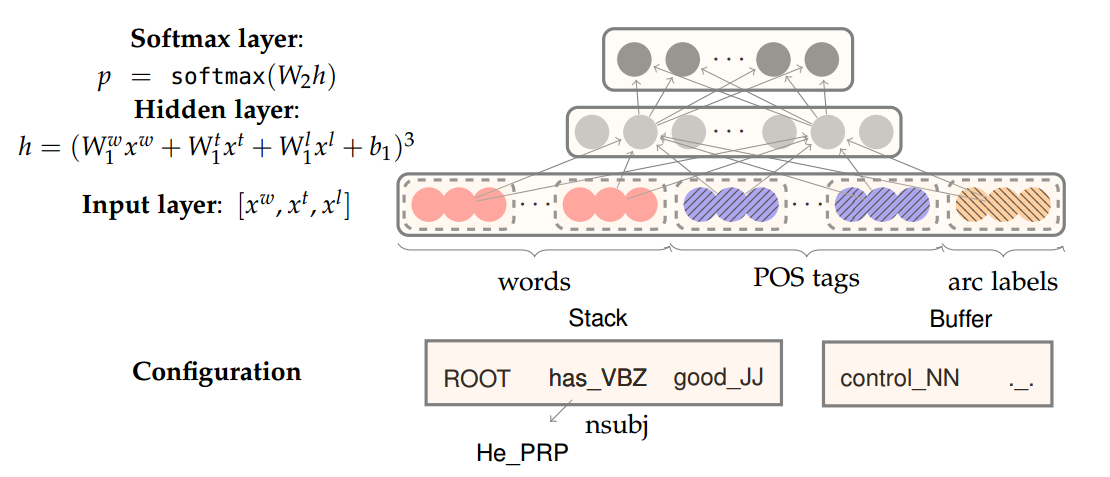
\includegraphics[width = 0.8\textwidth]{chap-04/04-model.png}
\caption{一个简单的神经网络,用来决策转移动作。网络依次包括嵌入层/输入层、隐层和softmax输出层。}
\label{04-net}
\end{figure}

模型最基础的结构如图\ref{04-net}所示。输出向量的维度和转移操作的种类数对应(3维),指出应该采取哪种转移。\cite{04-manning}提出了更复杂的网络结构。在Transition-Based依存分析方面也有很多丰富的思考,比如\cite{04-cnblogs1}等等。
随着深度学习的发展,使用深度学习解决依存分析问题的探索层出不穷,笔者在此列举的资料也只是管中窥豹,仅做参考。

% \end{multicols}

\section{章节附录}

\subsection{成分语法 \\ Constituency Grammar}
\label{Constituency Grammar}

成分语法的思路就是设计一套文法,和实际的自然语言语法形成密切对应。在相关的研究中,成分语法、短语结构文法(Phrase Structure Grammar)和上下文无关文法(Context Free Grammar)通常指代相同的概念,即用产生式文法的观点来解析自然语言的语法结构。

具体而言,考虑自然语言中的各个层次,如词语、短语、成分、句子等,他们对应的抽象概念是词性、短语类型、成分类型和句子类型,这些不同层级、不同类型的概念之间的联系可以用产生式文法来体现。细节如下:

\begin{itemize}
    \item 词语:词语是句子语法解析的终点,同种词性的词语在句子中发挥的作用是相似的,而词性在产生式中充当终结符(或准终结符)。例如,在产生式$Adj. \ Modified \ N. \ Phrase \to Adj.+N.$中,可以设计成$N.$就是终结符,也可以设计成$N.\to apple | banana | \cdots$,而定义$apple$等词语为终结符。
    \item 短语:短语由更低级的单元(词语)组成,而本身也有特定意义(短语的语法结构),对应文法中的非终结符。例如,$Adj. \ Modified \ N. \ Phrase$的一个实例是$big apple$,$big$属于$Adj.$,$apple$属于$N.$
    \item 成分:和短语一样,成分也是“句子-成分-短语-词语”的语法层次中间的链结,对应非终结符。例如,名词短语$big apple$可以充当句子的主语$S.$.
    \item 句子:对应文法中的起始符号。
    \item 层次间关系:层次间关系可以用产生式描述。
    \begin{itemize}
        \item 词语组成短语:某一特定类型的短语可以由特定词性的词语按特定顺序组成,这种信息用产生式描述,比如$Adj. \ Modified \ N. \ Phrase \to Adj.+N.$
        \item 短语充当成分:产生式阐明句子成分由怎样的短语充当。比如$S. \to Adj. \ Modified \ N. \ Phrase$.
        \item 成分组成句子:产生式阐明句子的构成方法。比如$Sentence \to S. + Predicate + O.$.
    \end{itemize}
\end{itemize}

使用产生式文法描述这些概念的关系是很自然的思路,很好理解。将句子按文法规则进行规约,获得的语法树能清晰地体现句法结构。但是,成分语法难以应用于大规模数据集上句子语法结构的表示,原因如下:
\begin{itemize}
\item 语法树的嵌套结构没有直观的表示方法:依存关系树中的节点都是单词,所以可以用每个单词的被依存者表示整棵树;但成分语法树中单词都是叶子节点,按照层次聚合起来,所以不好表示。
\item 智能方法无法学习新的规则,所有的文法规则需要由人提前定义好。考虑到大规模语料的复杂性,靠人力编排规则难免有遗漏和不周之处,而且和NLP目前通用化、智能化的趋势背道而驰。
\end{itemize}
综上所述,在大数据时代,语法结构表示上的弱点限制了成分语法的进一步应用和发展,目前的应用范围远不及依存语法。目前句子结构分析的大部分数据集都是基于依存关系建立的。

不过,成分语法作为一个形式优雅、定义清晰的概念,还是有很大用处的。比如,在缺数据的时候可以用成分语法生成一些句子数据,然后用生成的数据集验证模型。根据具体的生成方式,这些句子实际上属于几个特定的类别,所以有一定复杂性,适合作为验证数据。

\section*{章节未尽之处}

\begin{thebibliography}{本章节参考文献\&阅读材料}
\bibitem[notes04]{04-this_notes} \url{https://web.stanford.edu/class/cs224n/readings/cs224n-2019-notes04-dependencyparsing.pdf}
\bibitem[lecture05]{04-this_slides} \url{https://web.stanford.edu/class/cs224n/slides/cs224n-2019-lecture05-dep-parsing.pdf}
\bibitem[Phrase Structure Grammar]{04-phrase-struct-gram} \url{https://www.thoughtco.com/phrase-structure-grammar-1691509}
\bibitem[依存分析:中文依存句法分析简介]{04-blog1} \url{https://blog.csdn.net/sinat_33741547/article/details/79258045}
\bibitem[依存句法分析:原理、应用]{04-blog2} \url{https://blog.csdn.net/qq_17832003/article/details/84396257}
\bibitem[Dependency Parsing的两种解决方案]{04-cnblogs1} \url{https://www.cnblogs.com/zeze/p/9752734.html}
\bibitem[Nivre's Paper]{04-NivrePaper} Nivre, Joakim. (2019). Inductive Dependency Parsing of Natural Language Text. 
\bibitem[Nivre's Slides]{04-NivreSlides} \url{https://www.docin.com/p-1736992284.html}
\bibitem[Danqi Chen and Manning's Paper of Neural Dependency Parsing]{04-manning} Danqi Chen, and Christopher D. Manning. "A Fast and Accurate Dependency Parser using Neural Networks." EMNLP. 2014.
\bibitem[Nivre's Summary]{04-NivreP} Kuebler, Sandra, Ryan McDonald, and Joakim Nivre. “Dependency parsing.” Synthesis Lectures on Human Language Technologies 1.1 (2009): 1-127.
\bibitem[依存句法分析与语义依存分析的区别]{04-cnblogs2} \url{https://www.cnblogs.com/CheeseZH/p/5768389.html}
\bibitem[统计自然语言处理]{04-tj} 统计自然语言处理(第2版),宗成庆,ISBN: 9787302165989,引用3.2.1的内容.
\bibitem[Universal Grammar in Wikipedia]{04-uni1} \url{https://en.wikipedia.org/wiki/Universal_grammar}
\bibitem[What is Universal Grammar?]{04-uni2} \url{https://www.sohu.com/a/223760135_652705}
\bibitem[Definition and Examples of Universal Grammar (UG)]{04-uni3} \url{https://www.thoughtco.com/universal-grammar-1692571}
\bibitem[普遍语法假说学习汇报]{04-uni4} \url{https://wenku.baidu.com/view/654273093a3567ec102de2bd960590c69ec3d80f.html}
\end{thebibliography}


